%!TEX root = ../report.tex

\begin{document}
\appendix
\definecolor{eclipseGreen}{RGB}{63,127,95}
\definecolor{mypurple}{RGB}{102,0,153}
\definecolor{pythongreen}{rgb}{0,128,128}
\definecolor{pythonblue}{rgb}{0,0,128}
\newcommand{\ra}[1]{\renewcommand{\arraystretch}{#1}}
\newcommand{\lstsetpython}{
 \lstset{
        language=Python,
        breaklines=true,
        commentstyle=\textit,
        keywordstyle=\color{pythonblue},
        keywordstyle=[2]{\color{mypurple}},
        basicstyle=\ttfamily,
        stringstyle=\color{pythongreen},
        showstringspaces=false,
        frame=single,
        captionpos=b,
        morekeywords = [2]{local_dict, global_dict, evaluate},
        autogobble=true,
        %linewidth=\textwidth,captionpos=b
        %numbers=left, stepnumber=5, numbersep=10pt
 }
}
\chapter{Equation checking with Sympy}
\lstsetpython
\begin{lstlisting}[captionpos=b, caption=Comparing two equations, label={equationcheck}]
    if(simplify(eq1-eq2) == 0):
\end{lstlisting}
\lstsetpython
\begin{lstlisting}[captionpos=b, caption=Sympy Comparing Two Sets, label=comparingtwoset]
    if(isinstance((eq2 - eq1),EmptySet)):
\end{lstlisting}

\begin{figure}[h]
    \centering
    \usetikzlibrary{matrix}
        \begin{tikzpicture}[->]
            \tikzset{square matrix/.style={
                matrix of nodes,
                column sep=-\pgflinewidth, row sep=-\pgflinewidth,
                nodes={draw,
                  minimum height=#1,
                  anchor=center,
                  text width=#1,
                  align=center,
                  inner sep=0pt
                },
              },
              square matrix/.default=1.45cm
            }
              border/.style={draw}

              \matrix(vector)[square matrix]
              {
                  $i_{0}$\\
                  $i_{1}$\\
                  $\vdots$\\
                  $i_{7}$\\
              };
            \node(eq0) [left] at (-3,-0.2) {$P(W|S)$};
            \path[every node/.style={font=\sffamily\small}]
                (vector-1-1) edge[bend right] node [left] {} (eq0);
%                (vector-2-1) edge[bend right] node [left] {} (eq0)
%                (vector-3-1) edge[bend left] node [left] {} (eq0)
%                (vector-4-1) edge[bend left] node [left] {} (eq0);
        \end{tikzpicture}
    \caption{Array for storing the input}
    \caption*{Here a one dimensional array in which the input is stored which is checked against the initial equation can be seen.
    As soon as the input is entered the equation is transformed and checked against the initial equation.}\label{fig:CheckArray}
\end{figure}

\chapter{First approach for equation checking}
\lstsetpython
\begin{lstlisting}[captionpos=b, caption=Comparing two equations, label={equationcheck}]
    if(simplify(eq1-eq2) == 0):
\end{lstlisting}
\lstsetpython
\begin{lstlisting}[captionpos=b, caption=Sympy Comparing Two Sets, label={checkforemptyset}]
    if(isinstance((eq2 - eq1),EmptySet)):
\end{lstlisting}
\begin{lstlisting}[captionpos=b, caption=Creating a random symbol in Sympy, frame=single, label={randomsymbol}]
    sizeOfDice = 6
    X = Die('X', sizeOfDice)
    Y = Die('Y', sizeOfDice)
\end{lstlisting}
\begin{lstlisting}[captionpos=b, caption=Creating a finite random variable in Sympy, frame=single, label={finiterandomvariable}]
    S = Y >= 3
    W = X > 3
\end{lstlisting}
\begin{lstlisting}[captionpos=b, caption=Transforming a finite random variable into a set, frame=single, label={wherefunction}]
    Sset = where(S).set // gives {3, 4, 5, 6}
    Wset = where(W).set // gives {4, 5, 6}
\end{lstlisting}
\begin{lstlisting}[captionpos=b, caption=Transforming a finite random variable into a set, frame=single, label={negationofset}]
    // ~negates the set
    Sset = where(~S).set // gives {1, 2}
    Wset = where(~W).set // gives {1, 2, 3}
\end{lstlisting}
\begin{lstlisting}[captionpos=b, caption=A global dictionary in Sympy, frame=single, label={globaldict}]
    global_dict = {'P':P, 'Mul':Mul}
\end{lstlisting}
\begin{lstlisting}[captionpos=b, caption=A local dictionary in Sympy, frame=single, label={localdict}]
    local_dict={'S':S, 'W':W}
\end{lstlisting}
\begin{figure}[h]
    \begin{center}
        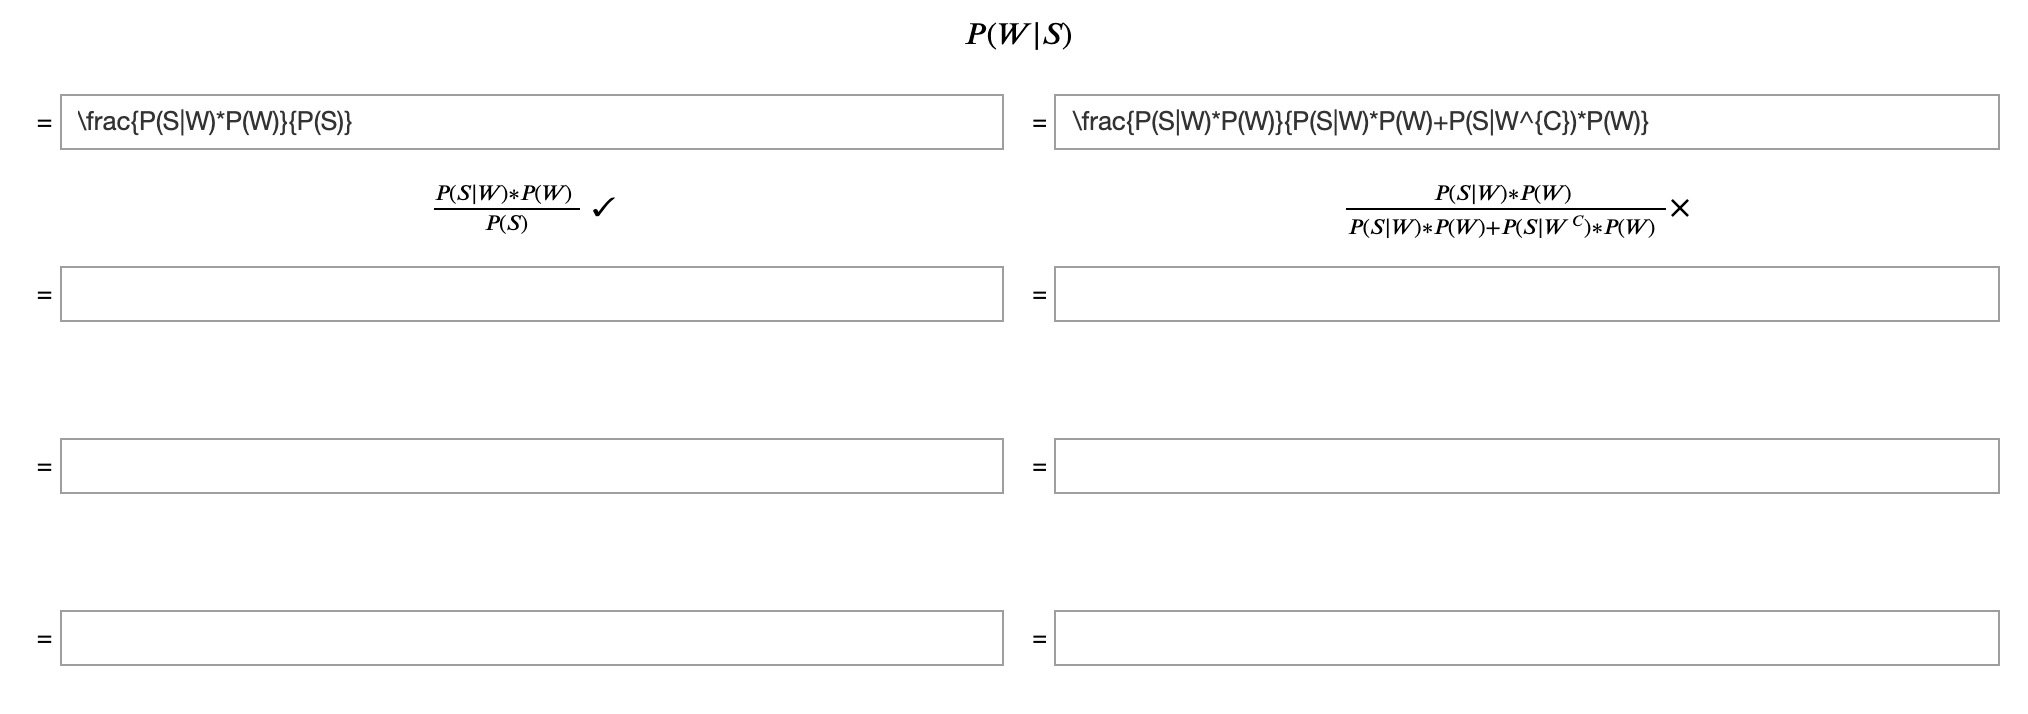
\includegraphics[scale=0.2]{./images/GridWithCorrection.jpg}
    \end{center}
    \caption{Grid in which students enter their equations}\label{fig:GridWithSolution}
\end{figure}
\chapter{Latex Parser}
\begin{table*}[h]\centering
    \ra{1.3}
    \begin{tabular}{c c}
    Input & Output \\
     \hline
     \textbf{\{} &  \textbf{(} \\
     \textbf{\}} & \textbf{)}\\
     $W^{C}$ & \text{\textasciitilde W}\\
     \textbf{|} & \textbf{,} \\ \bottomrule
    \end{tabular}
    \caption{Mapping of chars}\label{Mapping of chars}
\end{table*}
\chapter{Equation checking using finite random variables}
\begin{IEEEeqnarray*}{rCl}
    P(S \cap W)&=&P(S|W) \cdot P(W) \IEEEyesnumber \label{eq:-1} \\ \\
    &=&\frac{n_{ij}}{r_{j}} \cdot \frac{r_{j}}{N} \\ \\
    &=&\frac{n_{ij}}{N} \\ \\ \\
    P(S|W^{C})&=&\frac{P(W^{C}|S)P(S)}{P(W^{C})} \IEEEyesnumber \label{eq:-2} \\ \\
    &=&\frac{(1 - P(W|S))P(S)}{1 - P(W)} \\ \\
    &=&\frac{(1 -\frac{n_{ij}}{c_{i}})\frac{c_{i}}{N}}{1 - \frac{r_{j}}{N}} \\ \\ \\
    \frac{P (S \cap W^{C})}{P(W^{C})}&=&\frac{P(S) - P(S \cap W)}{1 - P(W)} \IEEEyesnumber \label{eq:-3} \\ \\
    &=&\frac{\frac{c_{i}}{N} - \frac{n_{ij}}{N}}{1 - \frac{r_{j}}{N}}
\end{IEEEeqnarray*}
\begin{figure}[h]
    \begin{center}
        \[\textbackslash frac\,\{P(S|W)*P(W)\}\{P(S|W)*P(W)+P(S|W\textasciicircum\{C\})*P(W\textasciicircum\{C\})\}\]
%        \[\rightarrow \frac{\frac{n_{ij}}{r_{j}} \cdot \frac{r_{j}}{N}}{\frac{n_{ij}}{r_{j}} \cdot \frac{r_{j}}{N}+\frac{(1 - \frac{n_{ij}}{c_{i}})*\frac{c_{i}}{N}}{1 - \frac{r_{j}}{N}}*(1 - \frac{r_{j}}{N})}\]
        \[\rightarrow (n/r*r/N)/(n/r*r/N+((1 - n/c)*c/N)/(1 - r/N)*(1 - r/N))\]
    \end{center}
    \caption{Application of dedicated Sympy parser} \label{fig:Application of dedicated extended Sympy parser}
\end{figure}

\end{document}
